\section{Using Cisco}\label{sec:cisco_usage}
The Cisco localisation and positioning system is already in use at Aalborg University. To be able to use the information from the system, we had a meeting with the administrator, during which he raised concerns for privacy, because of the legality of storing person sensitive data, as mentioned in \cref{sec:permission}. Furthermore he wishes to be able to provide the location data to future student projects with ease. To accommodate this, it has been asked of us to build and deploy an intermediate service with the goal of obfuscating sensitive personal data, such as MAC-addresses and user names. This service is intended to duplicate the functionality of the Cisco MSE RESTful API, such that the service acts as a transparent proxy. This is achieved by creating an intermediate RESTful service, that simply redirects requests and processes the response before sending it back to the initial requester, as illustrated on \cref{fig:cisco_usage}.

\begin{figure}[ht]
	\begin{center}
	\includegraphics[scale=0.9]{graphics/cisco_usage.png}
	\caption{Cisco usage}
	\label{fig:cisco_usage}
	\end{center} 
\end{figure}

A RESTful service typically communicates using the HTTP or HTTPS protocols, and functions by receiving requests for specific data resources, called Uniform Resource Identifiers (URIs) to which it responds by sending the requested data. As an example we can send a HTTPS GET request to 64.103.26.61, which is a Cisco MSE test server, with the URI "/api/contextaware/v1/location/clients" and, given that we supply the correct user name and password, receive a string of data corresponding to the type of request \cite{restful_oracle}.

To create a transparent RESTful service that duplicates the functionality of the Cisco RESTful API, we need to make use of the same URIs as the Cisco API\cite{cisco_mse_api}. This is done with the use of the Jersey Java library, which affords the possibility of creating a HTTP server and specifying what URIs are available for a client to request.

\begin{lstlisting}[caption={Adding a URI},label={lst:context_code},language=inc_Java]
server.createContext("/api/contextaware/v1/location/clients", httpExchange -> {
            if (VerifyConnection(httpExchange) == false){
                return;
            }

            String response = CollectAllClients(username, password, ciscoIp);
            httpExchange.sendResponseHeaders(200, response.length());
            OutputStream os = httpExchange.getResponseBody();
            os.write(response.getBytes(Charset.forName("UTF-8")));
            os.close();
        });
\end{lstlisting}
The code example shown on \cref{lst:context_code} shows an example of how to specify a URI. The createContext() method on line 1 takes two parameters: a string for the URI and an anonymous function implementing an interface. The anonymous function taking up the rest of the example dictates what actions are performed once a connection is established. In this case some verification is performed immediately after the function call, to authenticate the user. A response is generated based on the URI; on line 4 we retrieve all clients from Cisco using the ColletAllClients() function, which also performs the task of obfuscating necessary information. The list of clients is then written though an OutputStream to the requester, as seen on lines 8 and 9. The anonymous function terminates as the OutputStream is closed, which also serves as a termination of the HTTP connection. 

In order to accommodate the privacy concern, we implement some simple methods to obfuscate MAC-address and user name, one of which can be seen in \cref{lst:obfuscating_mac}. It might be the case that users allow for us to store their personal information, and as such we will have to make a check to see if this has been allowed. To store this information we use a TreeSet, which guarantees $log(n)$ time cost for adding, deleting and searching \cite{treeset}. On line 2 we obtain the MAC-address of the user, which is used on line 3 to perform a search in the TreeSet. If search returns empty we obfuscate the MAC-address, as seen on line 4. This is done in a similar way for the user name.

\begin{lstlisting}[caption={Obfuscating mac-address},label={lst:obfuscating_mac},language=inc_Java]
Private static Client ObfuscateMacAddress(Client singleClient) {
    String oldMacAddress = singleClient.getWirelessClientLocation().getMacAddress();
    if (!watchList.contains(oldMacAddress)) {
        singleClient.getWirelessClientLocation().setMacAddress(obfuscatedAddress);
    }
    return singleClient;
}
\end{lstlisting}

\subsection{System hierarchy}
With this code it is possible to create an intermediate service for the Cisco MSE RESTful service, that intercepts the response and obfuscates certain information. To use this service, a client needs to know the IP address and a login for the intermediate service. To automate the requests and create a flow of data from the Cisco systems to the aStep database, we will have to build and implement a client that fetches data at an interval. The scope of the project is beyond Aalborg University, and as such we want to integrate more than a single Cisco MSE system. 

\begin{figure}[ht]
	\begin{center}
	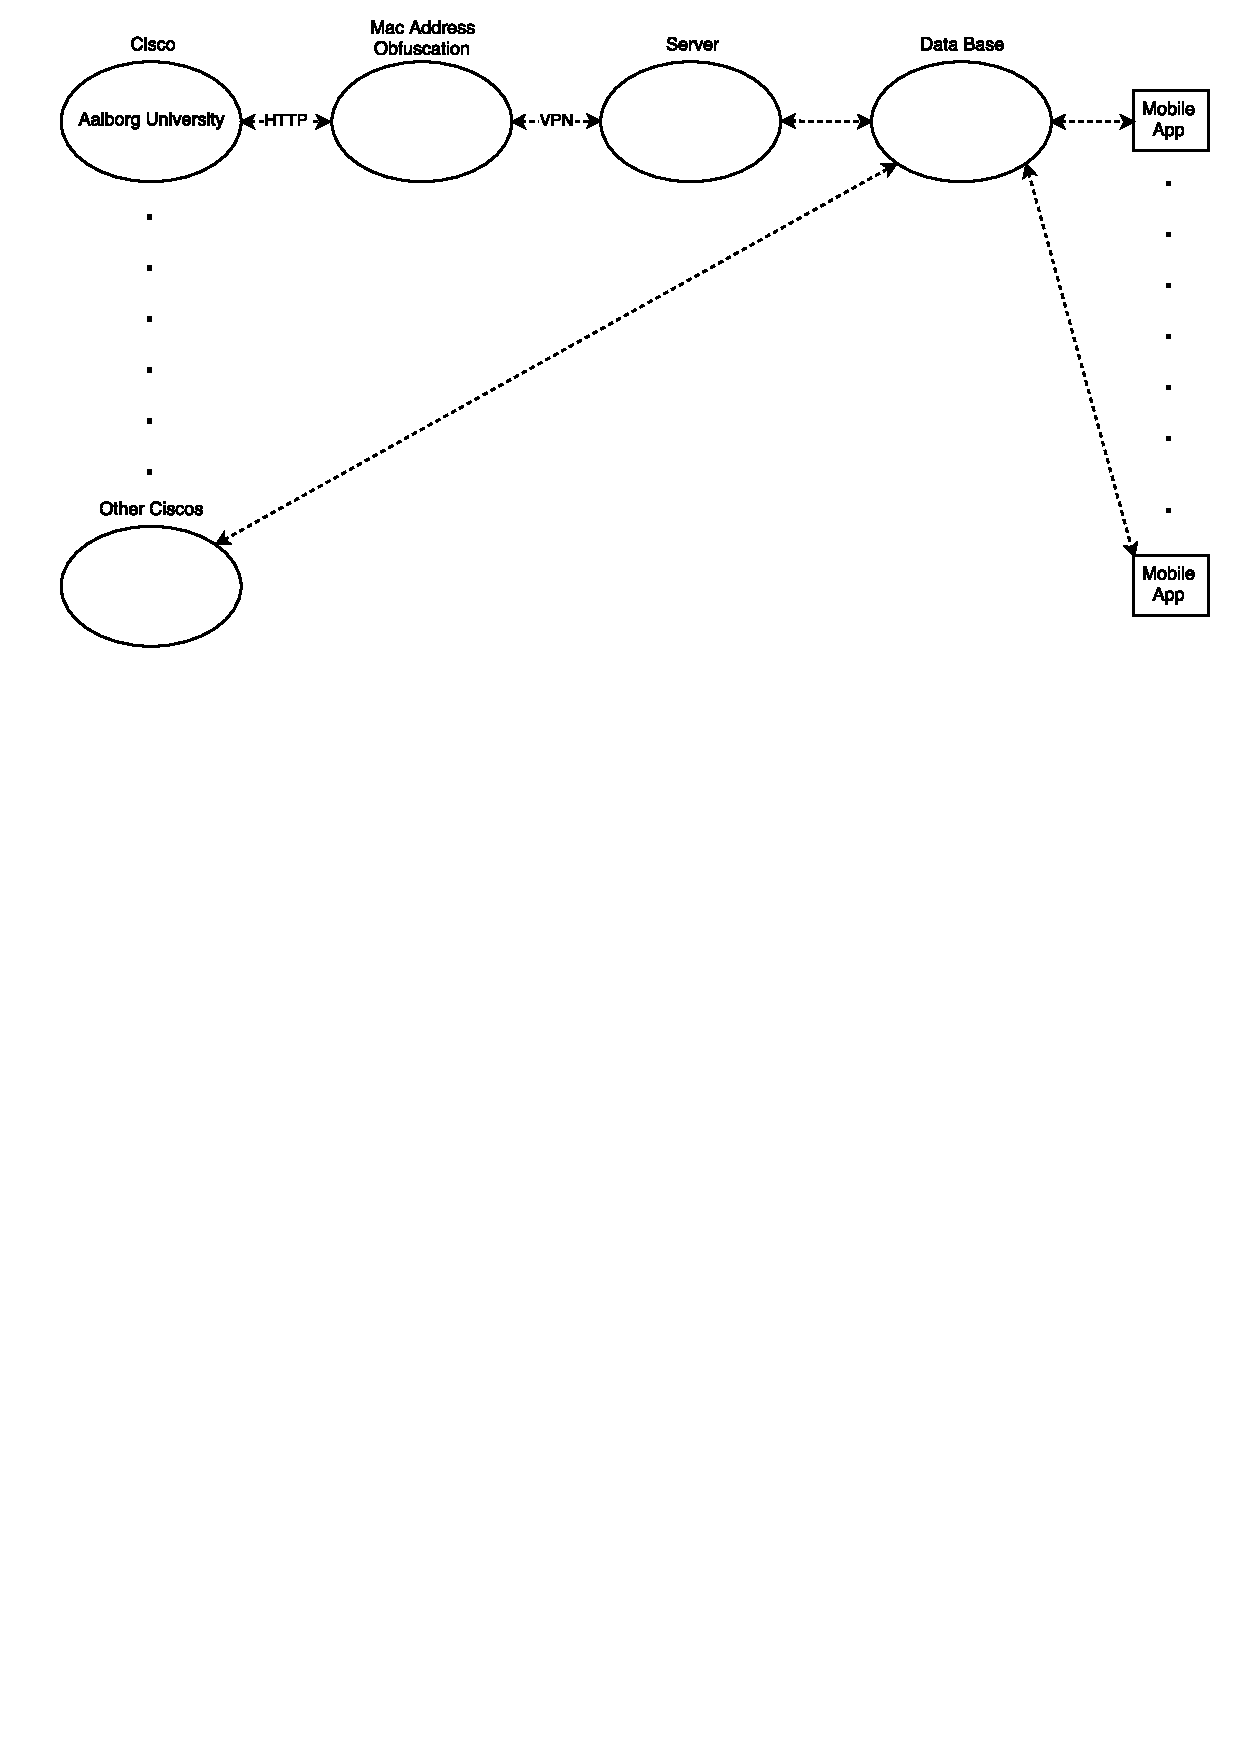
\includegraphics[scale=0.5]{graphics/ciscoSmall.pdf}
	\caption{Cisco systems}
	\label{fig:cisco_systems}
	\end{center} 
\end{figure}
\Cref{fig:cisco_systems} shows how the information flow is intended. The client connecting to the Cisco services can function as a server that requests data from all Cisco services that we have access to. Alternatively, a server can be implemented for each Cisco service. However, this solution has several downsides. First, it means corporations supplying the aStep project with information will have to have hardware running the server, which requires maintenance. Second, this solution is not scalable. The server running the aStep database will potentially be overloaded, as it has to handle each individual Cisco system sending information. As more Cisco systems are added, there will be less time to process received data. An alternative approach is to have the aStep database server request data, however, with an increase in connected Cisco systems, the interval at which we receive new information from a given system also increases. The optimal solution to this issue is to create a hierarchy of servers, such that the database server only receives data from a constant amount of intermediate servers, each of which also receive information from an amount of sources. During the start up of the aStep project we have access to a single Cisco MSE system, and as such we will not focus on building this hierarchy. However, as the project grows and additional Cisco systems are integrated, it will eventually become a necessity.  